% !TeX spellcheck = en_US
\chapter{Basic ML Problems}

\section{Linear Regression}
This is the simplest regression problem in \ac{ML}.

\hlb{Problem statement:} Given data points $\textbf{x}_i \in \mathbb{R}^D$ and their labels $y_i \in \mathbb{R}$, find the \textit{line} that fits these data points. The line is represented via parameters $\textbf{w} = [w_0, w_1, \dots, w_n]^T$. For each data point $\textbf{x}$ and its label $y$.

\hlb{Approach:}
\begin{align*}
	\bar{\textbf{x}} &= [1, x_0, \dots, x_n] && \text{(x bar - extended variable)}\\
	y \approx \hat{y} &= \bar{\textbf{x}} . \textbf{w} && \text{(y hat - predicted label)}\\
	\Rightarrow \frac{1}{2}e^2 &= \frac{1}{2} \left(y - \bar{\textbf{x}}.\textbf{w}\right)^2 && \text{(the squared error between true and predicted labels)}
\end{align*}
\begin{align}
	\mathcal{L}(\textbf{w}) &= \frac{1}{2} \sum_{i=1}^{N} \left(y_i - \bar{\textbf{x}}_i.\textbf{w}\right) ^2 && \text{(the loss function for all points)} \\
	\mathcal{L}(\textbf{w}) &= \frac{1}{2N} \sum_{i=1}^{N} \left(y_i - \bar{\textbf{x}}_i.\textbf{w}\right) ^2 && \text{(the average loss)} \\
	\textbf{w}^* &= \underset{\textbf{w}}{\text{argmin}}\,\mathcal{L}(\textbf{w}) && \text{(the weights that minimize the loss function)} \\
	\mathcal{L}(\textbf{w}) &= \frac{1}{2} ||\textbf{y}-\overline{\textbf{X}}.\textbf{w}||^2_2 && \text{(using matrix form)}
\end{align}

with $\overline{\textbf{X}} = \begin{bmatrix}
	\bar{\textbf{x}}_1 \\
	\bar{\textbf{x}}_2 \\
	\vdots \\
	\bar{\textbf{x}}_n
\end{bmatrix}$
and $\textbf{y} = \begin{bmatrix}
	y_1 \\
	y_2 \\
	\vdots \\
	y_n	
\end{bmatrix}$

\hlb{Solution:}
\begin{align}
	&\frac{\partial\mathcal{L}(\textbf{w}^*)}{\partial\textbf{w}} = \overline{\textbf{X}}^T \left( \overline{\textbf{X}} \textbf{w}^* - \textbf{y} \right) = 0 \\
	\Leftrightarrow \; &\overline{\textbf{X}}^T\overline{\textbf{X}}\textbf{w}^* = \overline{\textbf{X}}^T \textbf{y} \\
	\Leftrightarrow \; &\textbf{w}^* = \left( \overline{\textbf{X}}^T \overline{\textbf{X}} \right)^\dagger \overline{\textbf{X}}^T \textbf{y}
\end{align}
in which, $A^\dagger$ (A dagger) is the pseudo inverse of a matrix, because $A$ might not be inverse-able. {\color{red} \boxed{A^\dagger = \left(A^TA\right)^{-1}A^T}}\\

\note
\begin{itemize}
	\item Sensitive to outliers $\Rightarrow$ pre-processing
	\item Multi-variable:
	\begin{align*}
		\mathcal{L}(\textbf{w}) &= \frac{1}{2N} ||\textbf{y}-\overline{\textbf{X}}.\textbf{w}||^2_2 \\
		\Rightarrow\; \nabla_\textbf{w}\mathcal{L}(\textbf{w}) &= \frac{1}{N} \overline{\textbf{X}}^T (\overline{\textbf{X}}\textbf{w}-\textbf{y})
	\end{align*}
\end{itemize}
\section{Linear Discriminant Functions}
\label{sec:linear-classification}
\hlb{Problem statement:} of general classification problem
\begin{itemize}
	\item Given: training set $\textbf{X} = \{\textbf{x}_1, \textbf{x}_2, \dots, \textbf{x}_N\}$ with target values (labels) $\textbf{T} = \{\textbf{t}_1, \textbf{t}_2, \dots, \textbf{t}_N\}$.
	\item Goal: take a new input $\textbf{x}$ and assign it to one of $K$ classes $C_k$\\
	$\Rightarrow$ Learn a discriminant function $y(x)$ to perform the classification
\end{itemize}
\hlb{Approach:}
\begin{itemize}
	\item 2-class problem: Binary target values: $t_n \in \{0, 1\}$\\
	\Eg of discriminant function: $y(x) > 0 \Rightarrow$ class $C_1$, else $C_2$
	\item K-class problem: 1-of-K coding scheme, \eg: $\textbf{t}_n = [0, 1, 0, 0, 0]^T$
	\item Extension to multiple classes: one-vs-all, one-vs-one classifiers
\end{itemize}
\subsection{Least-Squares Classification}
With above problem statement, consider $K$ classes described by linear models:
\begin{align*}
	y_k(\textbf{x}) &= \textbf{w}^T_k\textbf{x} + w_{k0} && k=1, \dots, K \\
	\Rightarrow \textbf{y}(\textbf{x}) &= \widetilde{\textbf{W}}^T\widetilde{\textbf{x}} && \text{(using vector notation)} \\
	\textbf{Y}(\widetilde{\textbf{X}}) &= \widetilde{\textbf{X}}\widetilde{\textbf{W}} && \text{(for the entire dataset)}
\end{align*}
In which output $\textbf{y}$ in 1-of-K notation, and can be compared to the target value
\[\textbf{t}=[t_1, \dots, t_k]^T\]
\hlb{Solution:} minimize the sum-of-squares error $E(\textbf{w})$
\begin{align*}
	E(\textbf{w}) &= \frac{1}{2} \sum_{n=1}^{N} \left(\textbf{y} - \textbf{t}\right)^2 = 
	\frac{1}{2} \sum_{n=1}^{N} \sum_{k=1}^{K} \left(\textbf{w}_k^T\textbf{x}_n-t_{kn}\right)^2 \\
	\Rightarrow \widetilde{\textbf{W}}^* &=  \left( \widetilde{\textbf{X}}^T \widetilde{\textbf{X}} \right)^{-1} \widetilde{\textbf{X}}^T T = \widetilde{\textbf{X}}^\dagger T
\end{align*}
\note Least-squares is very sensitive to outliers!\\
The error function penalizes predictions that are “too correct”.

\subsection{Generalized Linear Discriminant}
\begin{equation}
	y_k(x) = \sum_{j=1}^{M}w_{kj}\phi_j(x) + w_{k0} = \sum_{j=0}^M w_{kj}\phi_j(x), \tab \phi_0(x) = 1
\end{equation}

\subsection{Generalized Linear Models}
\begin{itemize}
	\item Linear Model:
	\begin{equation}
		y(\textbf{x}) = \textbf{w}^T\textbf{x} + w_0
	\end{equation}	
	\item Generalized Linear Model:
	\begin{equation}
		y(\textbf{x}) = g(\textbf{w}^T\textbf{x} + w_0)
		\label{eq:generalized-linear-model}
	\end{equation}	
	In which $g(\cdot)$ is called an \hlb{activation function} and may be nonlinear
\end{itemize}

\section{Logistics Regression}

Though named as "regression", logistics regression is used for classification problem, just like Linear Discriminant (\secref{sec:linear-classification}).

\hlb{Problem:} In many of binary classification problems (classification problem with 2 classes), it's rather hard (or even impossible) to be certain about the class of the output, and the training data is not linear separable. Instead of a hard threshold, we could have a soft one, represent by the \ac{prob} belonging to either classes.
\begin{figure}[hbt!]
	\centering
	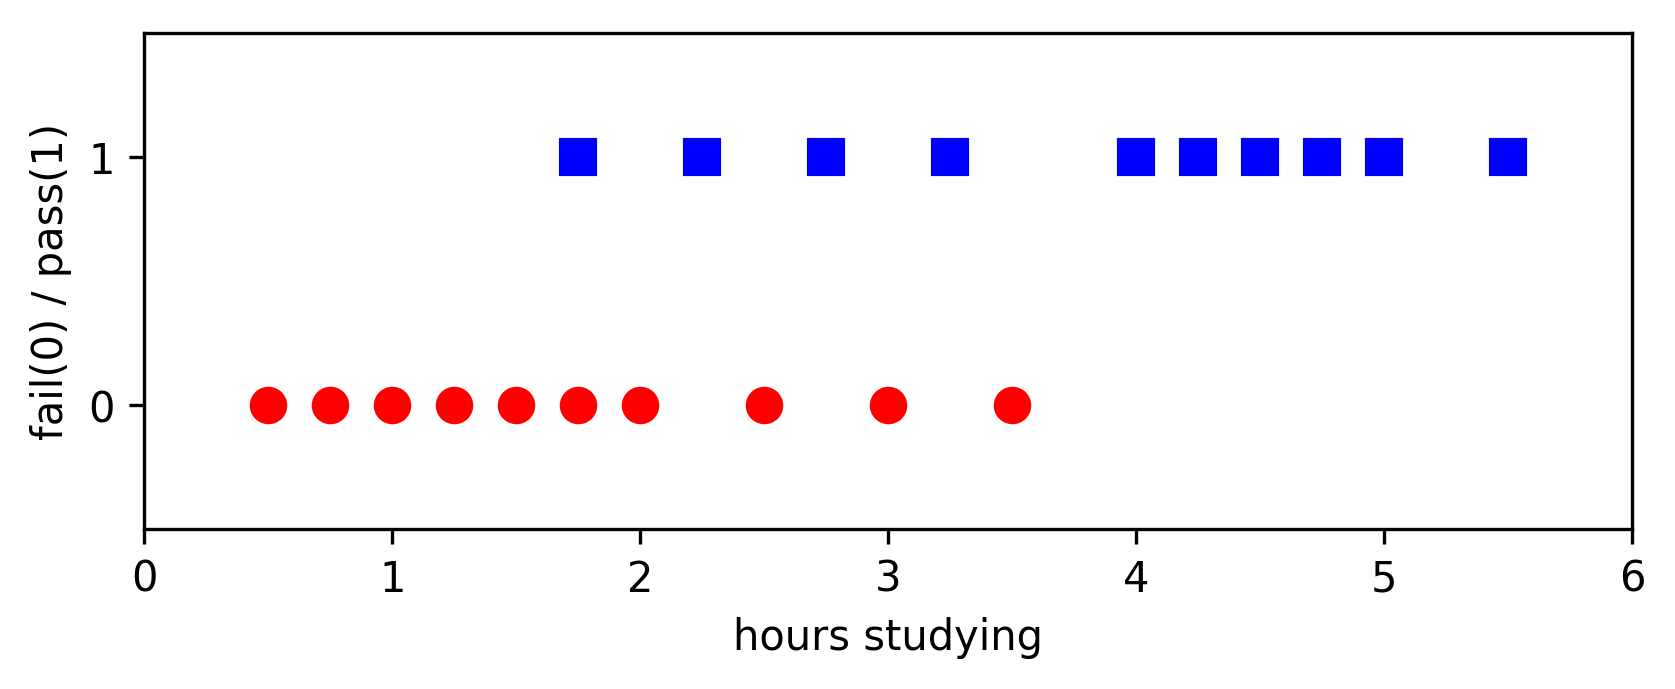
\includegraphics[width=0.79\textwidth]{sigmoid-example.png}
	\caption{Example of exam results based on study hours (\href{https://machinelearningcoban.com/2017/01/27/logisticregression/}{src}). Given the number of hours, instead of predicting whether fail or pass, the model predicts the \ac{prob} that the student will pass, or fail.}
\end{figure}

The sigmoid function gives a nice nonlinear transition for the \ac{prob}. The further the data point is from the threshold, the higher the \ac{prob} it belongs to one class, and small to the others.
\begin{align}
	f(s) 		&= \frac{1}{1 + e^{-s}} \overset{\triangle}{=} \sigma(s) \\
	s 			&= \text{ln} \left( \frac{\sigma}{1-\sigma} \right) \\
	\sigma'(s)	&= \sigma(s) \left( 1- \sigma(s) \right)
\end{align}
Thus, if we use the sigmoid function as the activation function for \eqref{eq:generalized-linear-model}:
\begin{align}
	s &= \textbf{w}^T \textbf{x} \\
	y &= \sigma(s)\\
	\Rightarrow \; \frac{\partial y}{\partial \textbf{w}}&= \frac{\partial y}{\partial s} \frac{\partial s}{\partial \textbf{w}} = y(1-y) \textbf{x}
	\label{eq:sigmoid}
\end{align}
\begin{figure}[hbt!]
	\centering
	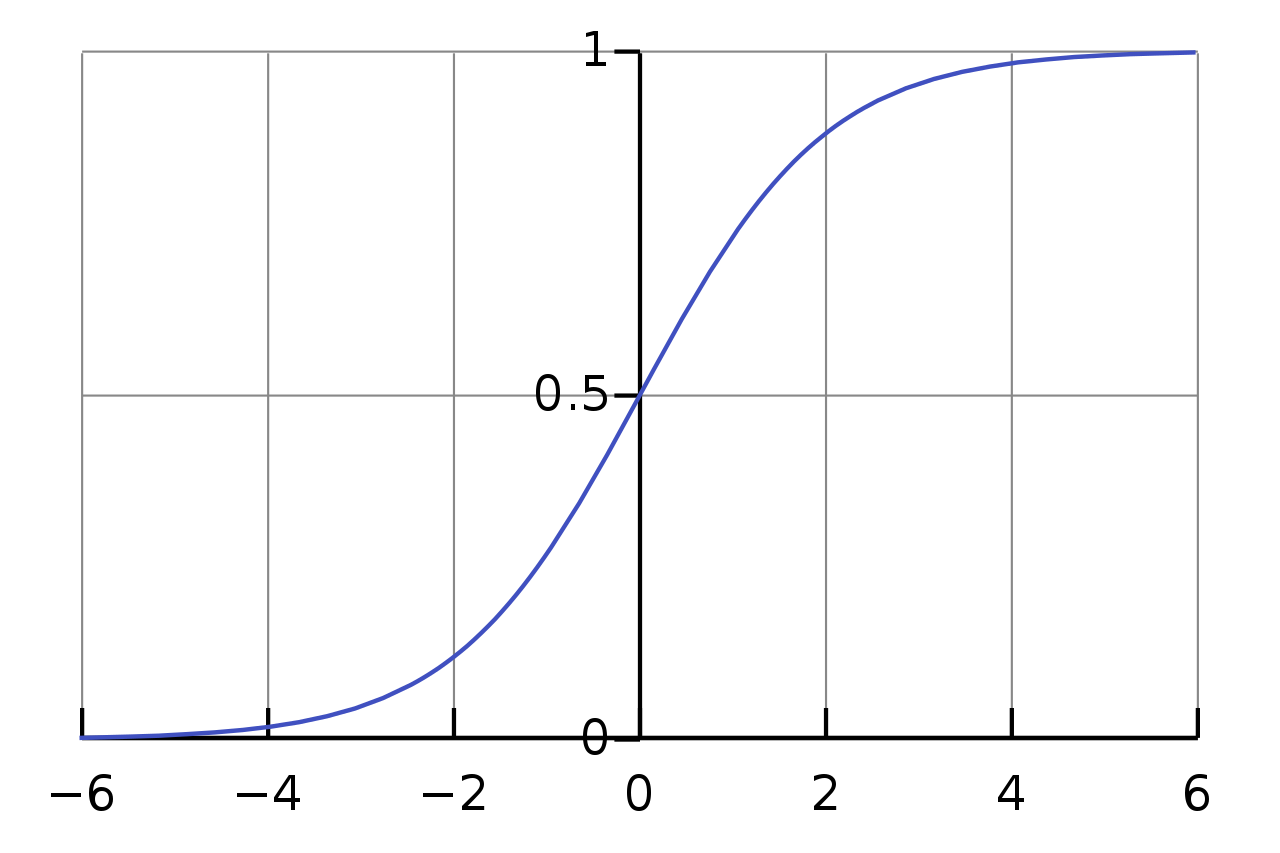
\includegraphics[width=0.5\textwidth]{sigmoid.png}
	\caption{Sigmoid function (\href{https://en.wikipedia.org/wiki/Sigmoid_function}{src}).}
\end{figure}

\hlb{Approach:}
\begin{itemize}
	\item Design of the error function.\\
	Assume that the \ac{prob} of data point $\textbf{x}$ falls into class 1 is $f(\textbf{w}^T\textbf{x})$ and class 0 is $1-f(\textbf{w}^T\textbf{x})$. With $z_i = f(\textbf{w}^T\textbf{x}_i)$:
	\begin{equation}
		\begin{cases}
			P(y_i=1|\textbf{x}_i; \textbf{w}) &= f(\textbf{w}^T\textbf{x}_i) = z_i \\
			P(y_i=0|\textbf{x}_i; \textbf{w}) &= 1 - f(\textbf{w}^T\textbf{x}_i) =1 - z_i
		\end{cases} \Leftrightarrow P(y_i | \textbf{x}_i; \textbf{w}) = z_i^{y_i}(1-z_i)^{1-y_i}
	\end{equation}
	With the aim to find the model \ac{param} that maximizes the data \ac{prob} (\subsecref{subsec:mle}):
	\begin{align*}
		& \textbf{w}^* = \arg \underset{\textbf{w}}{\max}\;P(\textbf{y}|\textbf{X; w}) && \\
		\iff & \textbf{w}^* = - \arg \underset{\textbf{w}}{\min} \log P(\textbf{y}|\textbf{X; w}) && \text{(negative log-likelihood)} \\
		& P(\mathbf{y}|\mathbf{X}; \mathbf{w}) = \prod_{i=1}^N P(y_i| \mathbf{x}_i; \mathbf{w}) = \prod_{i=1}^N z_i^{y_i}(1 - z_i)^{1- y_i} && \text{(independence assumption)} \\
		\Rightarrow & - \log P(\textbf{y}|\textbf{X; w}) = - \sum_{i=1}^{N} [ y_i\log z_i + (1-y_1)\log (1-z_i) ] && \text{(the cross entropy error)}
	\end{align*}
	
	\item Optimization with \ac{SGD}:
	\begin{align}
		& \textbf{w} = \textbf{w} - \eta.\frac{\partial J}{\partial \textbf{w}}, \quad \text{($\eta$ as the learning rate)}
		\label{eq:log-reg-sgd}\\			
		& J(\textbf{w}, \textbf{x}_i, y) = -\left( y_i\log z_i + (1-y_i)\log(1-z_i) \right), \quad \text{data point $(\textbf{x}_i, y_i)$} \\
		\Rightarrow \; &\frac{\partial J}{\partial \textbf{w}} = - \left( \frac{y_i}{z_i} - \frac{1-y_i}{1-z_i} \right) \frac{\partial z_i}{\partial\textbf{w}} = \frac{z_i - y_i}{z_i(1-z_i)} \frac{\partial z_i}{\partial\textbf{w}} \\
		& \frac{\partial z_i}{\partial \textbf{w}} = z_i(1-z_i) \textbf{x}_i \tab \text{(the beauty of sigmoid function, \eqref{eq:sigmoid})} \\
		\Rightarrow \; &\frac{\partial J}{\partial \textbf{w}} = (z_i - y_i) \textbf{x}_i\\
		\Rightarrow \; &w = w + \eta (y_i - z_i) \textbf{x}_i \tab \text{(replace into \eqref{eq:log-reg-sgd})}
	\end{align}
\end{itemize}

\note Require less \ac{param}, only $D$ with $D$ as the \ac{no} dimensions, compared to Gaussians with $\displaystyle \left[\frac{M(M+5)}{2}+1\right]$ \ac{param}.

\section{Softmax Regression}

Softmax Regression is the generalization of Logistics Regression for multiple-class classification problem. Thus, it is also known as: \hlr{Multinomial Logistics Regression, Maximum Entropy Classifier}. Logistics Regression can only be applied for binary classification problem. Given $C$ classes, we would need multiple one-vs-all or one-vs-one classifiers. Softmax regression offers a better alternative.
\begin{align}
	&z_i = \textbf{w}^T \textbf{x}_i\\
	&a_i = \frac{\text{exp}(z_i)}{\sum_{j=1}^{C}\text{exp}(z_j)}\\
	&\begin{cases}
		a_i > 0, \tab a_i \text{ represents the \ac{prob} the input belongs to class }C_i\\
		\sum a_i = 1 \\
		z_m > z_n \iff a_m > a_n \quad \text{(order)}
	\end{cases}
\end{align}

There are cases that one output $z_i$ is significantly greater than the others, which will lead to numerical error while coding. In these cases, the following Softmax version is more stable:
\begin{equation}
	a_i = \frac{\text{exp}(z_i)}{\sum_{j=1}^{C}\text{exp}(z_j)} = \frac{\text{exp}(z_i - c)}{\sum_{j=1}^{C}\text{exp}(z_j - c)},\quad c = \underset{i}{\max}\;z_i
\end{equation}

For the one hot coding representation, for each input $\textbf{x}$, the softmax regression model calculate a output vector $\textbf{a} = \textbf{W}^T \textbf{x}$. The loss function will be build to represent the difference between output $\textbf{a}$ and the real label $\textbf{y}$. Vector $\textbf{a}$ itself is a \ac{prob} distribution of the input belongs to different classes. Instead of choosing the squared error function, cross-entropy is a better alternative to represent the difference between two \ac{prob} distributions (\secref{sec:cross-entropy}). As mentioned before, $\textbf{q} >0$, thus, we can't choose $\textbf{q} = \textbf{y}$.
\begin{align}
	&J(\textbf{W},\textbf{x}_i,\textbf{y}_i) = - \sum_{i=1}^{N} \sum_{j=1}^{C} y_{ij}\,\text{log}(a_{ij}) && \text{for each data point } (\textbf{x}_i, \textbf{y}_i) \\
	&\frac{\partial J_i(\textbf{W})}{\partial \textbf{W}} = \textbf{x}_i \textbf{e}_i^T = \textbf{x}_i (\textbf{a}_{i} - \textbf{y}_{i})^T && \text{(the gradient)}\\
	&\textbf{W} = \textbf{W} + \eta \textbf{x}_i (\textbf{y}_i - \textbf{a}_i)^T && \text{(\ac{SGD}, \href{https://machinelearningcoban.com/2017/02/17/softmax/}{machinelearningcoban.com})}
\end{align}

\section{SVM}

\ac{SVM}

\subsection{Hard Margin \ac{SVM}}

\hlb{Problem:} Give $N$ data points $\textbf{x}_i$ and their labels $y_i \in \{-1, 1\}$, find the line that separate these points into two classes while maximize the margin.

\begin{figure}[hbt!]
	\centering
	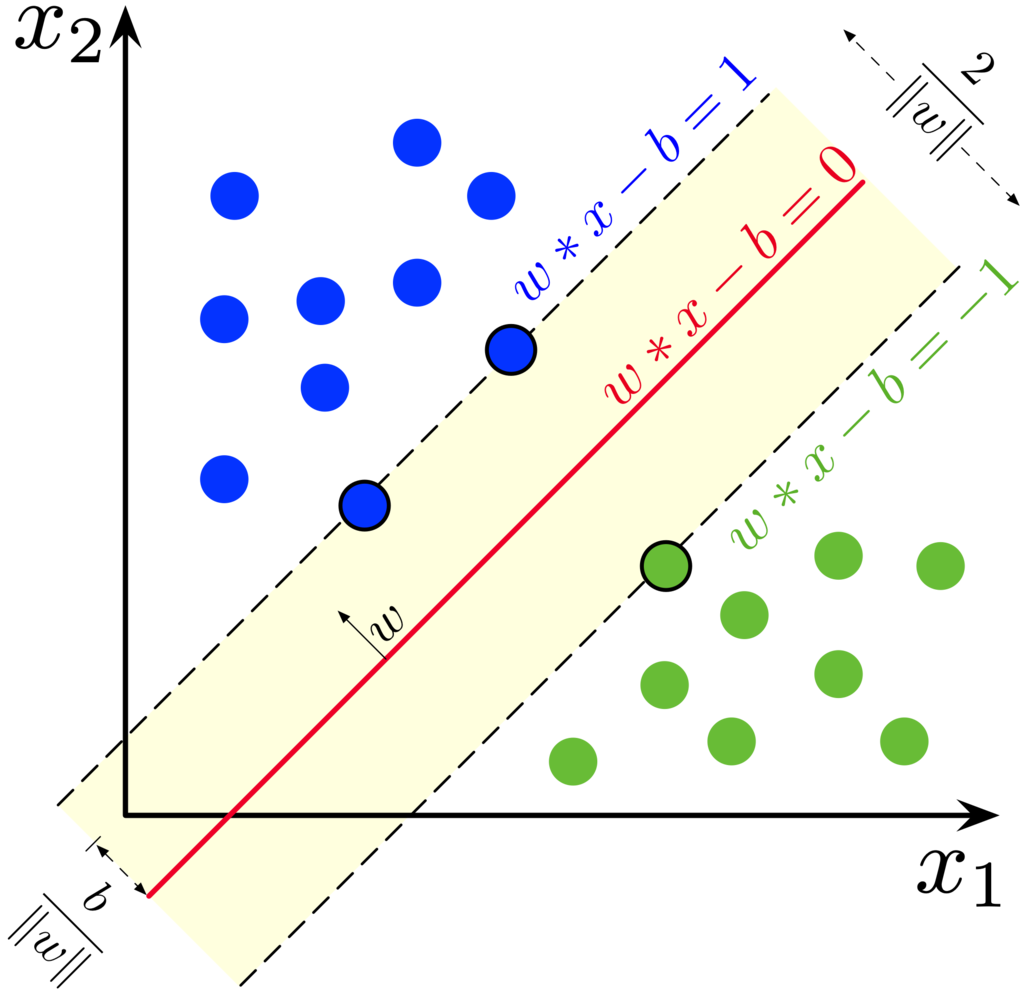
\includegraphics[width=0.5\textwidth]{svm.png}
	\caption{Example of \ac{SVM} (\href{https://en.wikipedia.org/wiki/Support-vector_machine}{src}).}
\end{figure}

\begin{align}
	&margin = \underset{n}{\min} \frac{y_n (\textbf{w}^T \textbf{x}_n) +b}{||\textbf{w}||_2}\\
	\Rightarrow\; &(\textbf{w},b) = \underset{\textbf{w}, b}{\arg\max} \left\{ \underset{n}{\min} \frac{y_n (\textbf{w}^T \textbf{x}_n) +b}{||\textbf{w}||_2} \right\} \\
	\Rightarrow\; &(\textbf{w},b) = \underset{\textbf{w}, b}{\arg\max} \left\{ \frac{1}{||\textbf{w}||_2} \underset{n}{\min}\left[ y_n(\textbf{w}^T \textbf{x}_n+b) \right] \right\}
\end{align}

For simplicity, we can assume that: $\underset{n}{\min}\left[ y_n(\textbf{w}^T \textbf{x}_n+b) \right] = 1$. Thus, the original problem can be transform to:

\hlb{Problem:} Find $\displaystyle (\textbf{w},b) = \underset{\textbf{w}, b}{\arg\min} \frac{1}{2}||\textbf{w}||^2_2$ that subject to:
\begin{equation*}
	1-y_n(\textbf{w}^T\textbf{x}_n+b) \leq 0, \quad \forall n = 1, 2, \dots, N
\end{equation*}
This is a well-studied optimization problem, solved with Lagrange's method.

\hlb{Approach:} The Lagrange's method

\hlr{The primal formulation of \ac{SVM}:}
\begin{align}
	& \mathcal{L}(\textbf{w}, b, \boldsymbol{\lambda}) = \frac{1}{2} ||\textbf{w}||^2_2 + \sum_{n=1}^{N} \lambda_n [1 - y_n(\textbf{w}^T\textbf{x}_n+b)], \quad \lambda_n \geq 0 \quad \forall n\\
	& \frac{\partial \mathcal{L}(\textbf{w}, b, \boldsymbol{\lambda})}{\partial\textbf{w}} = 0 \Rightarrow \textbf{w} = \sum_{n=1}^{N} \lambda_n y_n \textbf{x}_n \\
	& \frac{\partial \mathcal{L}(\textbf{w}, b, \boldsymbol{\lambda})}{\partial\textbf{b}} = 0 \Rightarrow \sum_{n=1}^{N} \lambda_n y_n =0
\end{align}
\hlr{The dual formulation of \ac{SVM}:}
\begin{align}
	\Rightarrow & g(\boldsymbol{\lambda}) = \sum_{n=1}^{N} \lambda_n - \frac{1}{2} \sum_{n=1}^{N} \sum_{m=1}^{N} \lambda_n \lambda_m y_n y_m \textbf{x}_n^T \textbf{x}_m \\
	\text{Set } & \textbf{V} = \left[ y_1\textbf{x}_1, y_2\textbf{x}_2, \dots, y_N\textbf{x}_N \right] \\
	\Rightarrow & g(\boldsymbol{\lambda}) = - \frac{1}{2} \boldsymbol{\lambda}^T \textbf{V}^T \textbf{V} \boldsymbol{\lambda} + 1^T\boldsymbol{\lambda} \qquad \text{is \hlb{concave} with} \quad \lambda_i \geq 0, \quad \sum_{n=1}^{N} \lambda_n y_n = 0
\end{align}
\hlr{$\Rightarrow$ Find $\lambda$ by solving Quadratic Programming}\\
Then use \ac{KKT} conditions to find $\textbf{w}, b$:\\
\hlre{S = \{n \;|\; \lambda_n \neq0\} \Rightarrow \begin{cases}
	b = \frac{1}{N_S} \sum_{n\in S} \left( y_n - \sum_{m \in S} \lambda_m y_m \textbf{x}_m^T \textbf{x}_n \right)\\
	\textbf{w} = \sum_{m \in S} \lambda_m y_m \textbf{x}_m
\end{cases}}

\subsection{Soft Margin \ac{SVM}}
\begin{itemize}
	\item Hard margin \ac{SVM}:
	\begin{align*}
		&(\textbf{w},b) = \underset{\textbf{w}, b}{\arg\min} \frac{1}{2}||\textbf{w}||^2_2 \\
		\text{subject to}\quad &y_n(\textbf{w}^T\textbf{x}_n+b) \geq 1 \quad \forall n
	\end{align*}
	\item Soft margin \ac{SVM}:
	\begin{align*}
		&(\textbf{w},b, \xi) = \underset{\textbf{w}, b, \xi}{\arg\min} \frac{1}{2} || \textbf{w} ||^2_2 + C \sum_{n=1}^{N} \xi_n \\
		\text{subject to}\quad &\begin{cases}
			y_n(\textbf{w}^T\textbf{x}_n+b) \geq 1 -\xi_n\\
			\xi_n \geq 0
		\end{cases} \quad \forall n 
	\end{align*}
\end{itemize}
\hlr{$C$ and the margins are in-proportional: $\begin{cases}
		C\uparrow \quad\Rightarrow\quad margin \downarrow \\
		C\downarrow \quad\Rightarrow\quad margin \uparrow
\end{cases}$}

The \textit{"Soft"} constraints:
\begin{equation*}
	y_n(\textbf{w}^T\textbf{x}_n+b) \geq 1 -\xi_n \quad \iff \quad 1 - \xi_n -y_n(\textbf{w}^T \textbf{x}_n +b) \leq 0 \quad \forall n
\end{equation*}

\hlb{Problem:} Find $\displaystyle (\textbf{w},b, \xi) = \underset{\textbf{w}, b, \xi}{\arg\min} \frac{1}{2} || \textbf{w} ||^2_2 + C \sum_{n=1}^{N} \xi_n$ that subject to:
\begin{equation*}
	\begin{cases}
		1 - \xi_n -y_n(\textbf{w}^T \textbf{x}_n +b) \leq 0 \\
		- \xi_n \leq 0
	\end{cases} \quad \forall n
\end{equation*}

\hlb{Approach:} Lagrange's method with $\lambda_i \geq 0$ and $\mu_i \geq 0$:
\begin{align}
	&\mathcal{L}(\textbf{w}, b, \boldsymbol{\xi, \lambda, \mu}) = \frac{1}{2} || \textbf{w} ||^2_2 + C \sum_{n=1}^{N} \xi_n + \sum_{n=1}^{N} \lambda_n [ 1-\xi_n - y_n(\textbf{w}^T \textbf{x}_n +b) ] - \sum_{n=1}^{N} \mu_n\xi_n \\
	&\frac{\partial \mathcal{L}}{\partial \textbf{w}} = 0 \iff \textbf{w} = \sum_{n=1}^N \lambda_n y_n \textbf{x}_n\\
	&\frac{\partial \mathcal{L}}{\partial b} = 0 \iff \sum_{n=1}^N \lambda_n y_n = 0\\
	&\frac{\partial \mathcal{L}}{\partial \xi_n} = 0 \iff \lambda_n = C - \mu_n\\
	&g(\boldsymbol{\lambda, \mu}) = \underset{\textbf{w}, b, \boldsymbol{\xi}}{\inf} \mathcal{L}(\textbf{w}, b, \boldsymbol{\xi, \lambda, \mu})\\
	\Rightarrow &g(\boldsymbol{\lambda, \mu}) = \sum_{n=1}^{N} \lambda_n - \frac{1}{2} \sum_{n=1}^{N} \sum_{m=1}^{N} \lambda_n \lambda_m y_n y_m \textbf{x}_n^T \textbf{x}_m = g(\boldsymbol{\lambda})\\
	\Rightarrow &\boldsymbol{\lambda} = \underset{\boldsymbol{\lambda}}{\arg\max} g(\boldsymbol{\lambda}) \quad \text{subject to} \quad \begin{cases}
		\sum_{n=1}^{N} \lambda_n y_n=0\\
		0 \leq \lambda_n \leq C \quad \forall n
	\end{cases}
\end{align}
After finding $\boldsymbol{\lambda}$:
\begin{align}
	&\mathcal{M} = \{ n \;|\; 0 < \lambda_n < C \} &&\Rightarrow b=\frac{1}{N_M} \sum_{n \in \mathcal{M}} \left( y_n - \sum_{m \in \mathcal{S}} \lambda_m y_m \textbf{x}_m^T \textbf{x}_n \right)\\
	&\mathcal{S} = \{ m \;|\; 0 < \lambda_m \leq C \} &&\Rightarrow \textbf{w} = \sum_{m \in \mathcal{S}} \lambda_m y_m \textbf{x}_m
\end{align}
\begin{itemize}
	\item $\begin{cases}
		\lambda_n =0\\
		\xi_n =0
	\end{cases} \Rightarrow$ \hlr{Safe points} 
	\item $\begin{cases}
		0 < \lambda_n < C\\
		\xi_n =0
	\end{cases} \Rightarrow$ \hlr{Marginal points} 
	\item $\lambda_n =C \quad \begin{cases}
		\xi_n  \leq 1 \quad\Rightarrow \text{\hlr{still correct}}\\
		\xi_n > 1 \quad\Rightarrow \text{\hlr{incorrect}}
	\end{cases}$
\end{itemize}

\subsection{Kernel Support Vector Machine}
\hlb{Mercer's Conditions:} kernel \ac{func} must theoretically satisfy.\\
In practice, however, some acceptable kernels don't satisfy the Mercer's conditions.
\begin{equation}
	\sum_{n=1}^N\sum_{m=1}^N k(x_n, x_m) c_n c_m \geq 0 \quad \forall c_i \in \mathbb{R}, i =1, 2, \dots, N
\end{equation}
\Eg kernel functions:
\begin{align*}
	&k(x,z) = x^T z && \hlr{linear}\\
	&k(x,z) = (\gamma x^T z + r)^d && \hlr{polynomial}\\
	&k(x,z) = \exp(-\gamma ||x-z||^2_2), \quad \gamma>0 && \hlr{\ac{RBF}}\\
	&k(x,z) = \tanh(\gamma x^T z + r) && \hlr{sigmoid}
\end{align*}

\chapter{Ensembles}
Ensemble of Models are also known as addictive models.

\section{Error Reduction}

\todo{Explanation}

\Eg: bagging
\begin{align}
	&y_{COM}(x) = \frac{1}{M} \sum_{m=1}^{M} y_m(x)\\
	&y(x) = h(x) + \varepsilon(x)\\
	&\mathbb{E}_x = \left[ y_m(x) - h(x) \right]^2 = \mathbb{E}_x \left[ \varepsilon_m(x)^2 \right]\\
	\Rightarrow &\mathbb{E}_{AV} = \frac{1}{M} \sum_{m=1}^{M} \mathbb{E}_x \left[ \varepsilon_m (x)^2 \right]\\
	&\mathbb{E}_{COM} = \mathbb{E}_x \left[ \left\{ \frac{1}{M} \sum_{m=1}^{M} y_m(x) - h(x) \right\}^2 \right] = \mathbb{E}_x \left[ \left\{ \frac{1}{M} \sum_{m=1}^{M} \varepsilon_m(x) \right\}^2 \right]
\end{align}

$\Rightarrow$ if $\begin{cases}
	\text{errors have 0 mean:} \qquad\qquad \mathbb{E}_x[\varepsilon_m(x)]=0\\
	\text{errors are uncorrelated:} \qquad \mathbb{E}_x[\varepsilon_m(x) \varepsilon_j(x)]=0 \text{ (unrealistic??)}
\end{cases} \Rightarrow \mathbb{E}_{COM} = \frac{1}{M} \mathbb{E}_{AV}$

However, in general, $\mathbb{E}_{COM} < \mathbb{E}_{AV}$

\note The weak classifiers have to be unstable algorithms, \ie, decision trees, neural network; \hlr{NOT} nearest neighbor, \ac{SVM}, linear regression.

\section{Bagging}
\label{sec:bagging}
\begin{itemize}
	\item Check \href{https://youtu.be/2Mg8QD0F1dQ}{Udacity's video}
	\item \ac{aka} Bootstrap aggregating
	\item Average $\approx$ 63\%
\end{itemize}

\todo{Image}
\begin{itemize}
	\item Split the given data set into train and test set
	\item Assume train set with $n$ data points
	\item Pick $n'$ data points into each bag $D_i$,\quad $\frac{n'}{n} < 1 (\approx 60\%)$
	\item Create $m$ data bags: $D_1, D_2, \dots, D_m$
	\item Learn a model $M_i$ from each bag $D_i$
	\item The final output is the average of models' outputs:
	\[y = \frac{1}{m} \sum_{i=1}^{m} f(M_i)\]
	\item \hlr{Random with replacement:} bag $i$ can have multiple times data point $\textbf{x}_i$
	\item \hlr{Simple, easy to implement, commonly used}
\end{itemize}
\note Practically, resampling with replacement is \hlb{usually unnecessary}, since \ac{SGD} and random initialization usually makes the models sufficiently independent.

\section{Boosting}
\begin{itemize}
	\item Adaboost
	\item Gradient boosting
	\item Xgboost (extreme gradient boosting)
	\item Gentle Boost (cross entropy error)
\end{itemize}

\subsection{Adaboost}
Resources:
\begin{itemize}
	\item \href{https://youtu.be/LsK-xG1cLYA}{AdaBoost, Clearly Explained}
	\item 
\end{itemize}

\begin{enumerate}
	\item First weak classifier
	\item Calculate error $J \Rightarrow \varepsilon$\\
	in case of normalization $w \Rightarrow \sum w = 1 \Rightarrow \varepsilon = J$
	\item Calculate amount of say $\alpha$ from $\varepsilon$
	\item Update $w$ with $\alpha$ (normalize $w$)
	\item 2nd weak classifier with new weight $w$ or sample on new $w$
\end{enumerate}

\begin{itemize}
	\item Ensembles of Classifiers: $K$ independent classifiers, error \ac{prob} < 0.5
	\item Suitable for unstable algorithms (\ie, decision trees, neural networks)
	\item Not good with stable methods (\ie, nearest neighbors, \ac{SVM}s, linear regression)
\end{itemize}

\todo{EXPLANATION?}
\begin{align}
	& -g(x_i) = -\frac{\partial \mathcal{L} (y_i, F(x_i))}{\partial F(x_i)} \\
	\Rightarrow & \text{Regression model: } \quad h_i \text{ for } (x_i, -g(x_i))\\
	\Rightarrow & F:= F + \rho h, \quad \rho = 1
\end{align}

\todo{EXPLANATION?}\\
\hlb{Problem:} \begin{itemize}
	\item Given: $N$ data points and their labels $(x_n, t_n)$
	\item Goal: find $M$ weak classifiers $h_m(x)$
\end{itemize}
\begin{align}
	w_n^{(0)} &= \frac{1}{N} && \text{initial data weights}\\
	J_m &= \sum_{n=1}^{N} w_n^{(m)} I\left( h_m(x) \neq t_n \right) && \text{weighted error function}\\
	\varepsilon_m &= \frac{\sum_{n=1}^{N} w_n^{(m)} I\left( h_m(x) \neq t_n \right) }{\sum_{n=1}^{N} w_n^{(m)}} && \text{(normalized) weighted error}\\
	\alpha_m &= \ln \left(\frac{1-\varepsilon_m}{\varepsilon_m}\right) && \text{classifier weights}\\
	w_n^{(m+1)} &= w_n^{(m)}.\exp\left\{ \alpha_m I\left( h_m(x) \neq t_n \right)\right\} && \text{updated data weights}\\
	H(x) &= sign\left( \sum_{m=1}^{M} \alpha_m h_m(x) \right) && \text{final classification}
\end{align}

\todo{EXPLANATION?}
\hlr{Adaboost}
\begin{align}
	&F(x) = sign \left( \sum_{m=1}^{M} \theta_m f_m(x) \right)\\
	&w(x_i, y_i) = \frac{1}{n} \qquad\qquad \text{initial weights for each data}\\
	&\varepsilon_m = \mathbb{E}_{\varepsilon_m} \left[ 1_{y \neq f(x)} \right]\\
	\Rightarrow\; &\theta_m = \frac{1}{2} \ln\left( \frac{1-\varepsilon_m}{\varepsilon_m} \right) \qquad\qquad \text{Update rule}\\
	&w_{m+1}(x_i, y_i) = \frac{w_m(x_i, y_i) \exp[-\theta_m y_i f_m(x_i)]}{z_m} \qquad\qquad \text{update weights}\\
	&(z_m \text{ is the normalization factor})
\end{align}

\todo{Explanation:}
\hlr{Exponential error used in Adaboost}
\begin{itemize}
	\item Fast convergence
	\item No penalty for too correct
	\item Less robust to outlier
\end{itemize}
\todo{Add function graph}

\subsection{Gradient Boosting (Regression)}
Check: A Gentle Introduction to Gradient Boosting - Cheng Li, CCS, Northeastern Uni
\begin{align}
	& (x_i, y_i) \text{ and first model } F_1(x)\\
	\Rightarrow & \text{ fit } F_2(x) \text{ to } (x_i, y_i - F_1(x_i)), \quad y_i - F_1(x_i)=h(x_i)	\text{ as the residuals}\\
	& J = \sum \mathcal{L} (y_i, F(x_i))\\
	\Rightarrow & F_{i+1} = F_i + h_i\\
	&{\color{red} \mathcal{L} = \frac{(y_i - F_i)^2}{2} \Rightarrow -g = y_i - F_i(x_i)} \\
	\label{eq:1}
	&{\color{red} \mathcal{L} = |y-F| \qquad \qquad \text{(absolute loss)} }\\
	\label{eq:2}
	&{\color{red} \mathcal{L} =\begin{cases}
			\frac{1}{2} (y-F)^2 \qquad\qquad \text{if } |y-F| \geq \delta\\
			\delta \left( |y-F| - \frac{\delta}{2} \right) \qquad \text{if } |y-F| <\delta
	\end{cases} \qquad \text{(Huber loss)}} 
\end{align}

The two loss functions \eqref{eq:1} and \eqref{eq:2} are less sensitive to outliers

\section{Information}

Mutual Information: \href{https://www.youtube.com/watch?v=d7AUaut6hso}{YouTube}, \href{https://www.youtube.com/watch?v=U9h1xkNELvY}{YouTube}.

\section{Decision Trees}

Iterative Dichotomiser 3: \href{https://machinelearningcoban.com/2018/01/14/id3/}{MLCoBan}
Detail Example calculation: \href{https://medium.com/@rishabhjain_22692/decision-trees-it-begins-here-93ff54ef134}{medium.com}, 
\href{https://clearpredictions.com/Home/DecisionTree}{blog}

CART: Gini Index: \href{http://www.learnbymarketing.com/481/decision-tree-flavors-gini-info-gain/}{blog}

Random forest: \href{https://www.youtube.com/watch?v=D_2LkhMJcfY}{YouTube}

\todo{Add image} root node, non-leaf node has 2 (or more) child node, leaf/terminal node. All non-leaf nodes have 2 child nodes $\Rightarrow$ binary decision tree

Iterative Dichotomiser 3 (ID3) only for categorical attribute (discrete)

Classification and Regression Tree (CART) for both categorical and continuous.

6 questions:
\begin{itemize}
	\item Bin / multi valued
	\item when node $\rightarrow$ leaf
	\item Deal impure nodes?
	\item how to select query
	\item pruned?
	\item missing attribute?
\end{itemize}

Impurity measures:
\begin{itemize}
	\item Misclassification: $i(s_j) = 1 - \underset{k}{\max}\;p(C_k | s_j)$
	\item Information gain: $C$ classes with $N_C$ as the number of members in each class
	\begin{equation}
		H(S) = - \sum_{c=1}^{C} \frac{N_C}{N} \log \left(\frac{N_C}{N}\right) \qquad \text{entropy at a node}
	\end{equation}
	Choose attribute $X$ $\Rightarrow$ $K$ child nodes: $S_1, S_2, \dots, S_k$ with $m_k$ elements
	\begin{align}
		&H(x, S) =  \sum_{k=1}^{K} \frac{m_k}{N} H(S_k) \qquad \text{entropy sum with weights} \\
		\Rightarrow\; &G(x, S) = H(S) - H(x, S) \qquad \text{information gain}\\
		&x^* = \underset{x}{\arg\max}\;G(x, S) = \underset{x}{\arg\min}\;H(x, S)
	\end{align}
	\hlr{Reduction in entropy = gain in information}
	\item Gini Index:
	\begin{align}
		i(s_j) &= \sum_{k \neq l} p(C_k | s_j) p(C_l, s_j) \qquad \text{variance impurity at node } s_j\\
		&= \frac{1}{2} \left[1- \sum_{k} p^2(C_k, s_j) \right]\\
		H(x, s_j) &= \sum_{k=1}^{K} \frac{m_k}{N} i(s_j)\\
		\Rightarrow x^* &= \min H(x, s_j)
	\end{align}
	\item Chi-square: $\displaystyle = \sqrt{\frac{(actual - expected)^2}{expected}}$, $\arg\max$\\
	CHAID: Chi-square Automatic Interaction Detector
	\item Reduction in Variance, $\arg\min$\\
	\begin{equation}
		i(s_j) = \frac{\sum (x-\bar{x})^2}{n}
	\end{equation}
\end{itemize}

\todo{Add image}

\hlr{Stopping and Pruning is more IMPORTANT}

\subsection{Stopping Conditions}
\begin{itemize}
	\item Prevent over-fitting = \hlr{Prepruning}
	\item $H(\mathcal{S}) = 0$: entropy $= 0 \Rightarrow \forall \text{ points } \in$ each class
	\item \ac{no} members in each node < a certain threshold\\
	The leaf node's class = the dominant class
	\item Distance from node $\rightarrow$ root $= c \Rightarrow$ to limit the tree depth
	\item The total \ac{no} of node exceed a threshold
	\item Further expansion induces insignificant entropy reduction
\end{itemize}

\subsection{Pruning}
\hlr{Post-pruning}
\begin{enumerate}
	\item Validation Set: Prune a node if it increases the \hlb{precision} for VS (Validation Set). This is also called Reduction error pruning method
	\item Regularized loss function
	\begin{equation}
		\mathcal{L} = \sum_{k=1}^{K} \frac{|\mathcal{S}_k|}{\mathcal{S}} H(\mathcal{S}_k) + \lambda K
	\end{equation}
	\begin{itemize}
		\item Minimum error: sensitive to \ac{no} classes, the least accurate in practice
		\item Pessimistic: the most crude and the quickest, no need for validation set, but extra caution needed
		\item Error complexity: $R(t) = r(t) p(t) + \alpha N_t$, with $r(t)$ as the error, $N_t$ as the \ac{no} leafs
		\item Critical value: the value we choose to decide the query at each nodes\\
		$\Rightarrow$ depends on how the tree is created
		\item Reduced error: \dots
	\end{itemize}
	\note The last three error functions are more stable and accurate
\end{enumerate}

\subsection{Computational Complexity}
Given:
\begin{equation*}
	\begin{cases}
		N \text{ data points}\\
		D \text{ dimensions}
	\end{cases} \Rightarrow \begin{cases}
	\text{Storage: } \mathcal{O}(N)\\
	\text{Test time: } \mathcal{O}(\log N)\\
	\text{Training time: } \mathcal{O}(DN^2 \log N)
	\end{cases}
\end{equation*}

\hlb{Explanation:}
\begin{itemize}
	\item Test time: in the worst case scenario, each leaf has one data\\
	$\Rightarrow$ After k step, the number of nodes are: $2^k = N$\\
	$\Rightarrow k \in \mathcal{O} (\log N)$
	\item Training time:\\
	maximum $\mathcal{O}(DN\log N)$ times each node\\
	maximum $N$ nodes
\end{itemize}

\subsection{Summary}
\begin{itemize}
	\item Simple
	\item Interpretable results
	\item Resistance to overfitting
	\item \hlr{Memory consumption $\Rightarrow$ suitable for problems with little data} 
	\item Noisy weak classifiers not generated well
	\item Sensitive to outliers \hlb{??}
	\item Expensive learning step
\end{itemize}

\section{Random Forest}
\begin{itemize}
	\item Handle missing values while maintaining accuracy
	\item Won't overfit
	\item Not good with regression
	\item Have little control to modify
\end{itemize}

Steps:
\begin{itemize}
	\item Sample from training set
	\item Choose $m<M$ (input features). At each node, select $m$ random data from $M$ to decide query attribute to split the node
	\item Grow tree to the largest, no pruning
	\item Predict data output:
	\begin{itemize}
		\item classification $\Rightarrow$ majority vote
		\item regression $\Rightarrow$ average
	\end{itemize}
\end{itemize}

Choose randomly $K$ attributes:\\
Training time: $\mathcal{O}(KN^2 \log N), \qquad K \ll D \qquad (K = \sqrt{N_\delta})$\\
Typically: $\begin{cases}
	K = 10 \qquad \text{root node}\\
	K=100 d \qquad \text{level-$d$ node}
\end{cases}$

\section{Bayesian Model Averaging}

Given $H$ different models with prior \ac{prob} $p(h)$, the final output would be the weighted average of these models:
\begin{equation}
	p(X) = \sum_{h=1}^{H} p(X|h)p(h)
\end{equation}

\section{Distillation}
\label{sec:distillation}
Ensemble models is usually more robust than single models. However, the big question is:\\
\hlb{Can we make a single model that is as good as an ensemble?}

$\Rightarrow$ \hlb{Distillation:} train on the ensemble's predictions as "soft" targets \cite{hinton2015distilling}
\begin{equation}
	p_i = \frac{\exp(z_i / T)}{\sum_j \exp (z_j / T)}
\end{equation}

\hlb{Intuition:} more knowledge in soft targets than hard labels!